\documentclass[12pt, a4paper, openany]{book}
\usepackage[italian]{babel}
\usepackage{listings}
\usepackage{graphicx}
\usepackage{fancyvrb}
\graphicspath{ {./images/} }
\renewcommand{\labelenumii}{\arabic{enumi}.\arabic{enumii}}

\begin{document}
\title{ADE - Archietettura degli elaboratori}
\author{Elia Ronchetti}
\date{Marzo 2022}

\maketitle
\tableofcontents

\chapter{Introduzione e Argomenti}
\section{Rappresentazione dell'informazione}
\begin{itemize}
    \item Sistemi numerici
    \item Rappresentazione dei numeri interi con e senza segno
    \item Rappresentazione dei numeri in virgola fissa e mobile
    \item Rappresentazione dell'informatica non numerica
\end{itemize}

\section{Circuiti logici}
\begin{itemize}
    \item Reti combinatorie
    \item Reti sequenziali e FSM (Finite State Machine)
    \item Rassegna di circuiti notevoli (decoder, multiplexer, register file, ALU, etc.)
\end{itemize}

\section{Instruction Set Architecture (ISA)}
\begin{itemize}
    \item schema di von Neumann
    \item CPU, registri, ALU e memoria
    \item Ciclo fondamentale di esecuzione di una istruzione (fetch/decode/execute)
    \item Tipi e formati di istruzioni MIPS32
    \item Modalità di indirizzamento
\end{itemize}

\section{Linguaggio Assembly}
\begin{itemize}
    \item Formato simbolico delle istruzioni
    \item Catena di programmazione (compilatore, assembler, linker, loader, debugger, etc.)
    \item Pseudo-istruzioni e direttive dell'assemblatore
    \item Scrittura di semplici programmi assembly
    \item Convenzioni programmative (memoria, nomi dei registri, etc.)
\end{itemize}

\section{Datapath}
\begin{itemize}
    \item Percorsi dei dati per le diverse classi di istruzioni
    \item Controllo del percorso dei dati con FSM
\end{itemize}

\section{Gestione delle eccezioni}
\begin{itemize}
    \item Tassonomia di eccezioni in terminologia MIPS32
    \item Modifiche alla FSM di controllo, registro Cause
\end{itemize}

\section{Tecniche di gestione dell'ingresso/uscita}
\begin{itemize}
    \item Controllo di programma
    \item Interruzione di programma
    \item Accesso diretto alla memoria
\end{itemize}

\section{Gerarchie di memoria: cache}
\begin{itemize}
    \item Cache a mappature diretta
    \item Cahce fully associative
    \item Cache n-way set associative
\end{itemize}

%Fine indice - Inizio Appunti

\chapter{Sistemi numerici} 

Con il termine bit definiamo l'unità di misura dell'informazione. Un bit può assumero solo il valore di 0 o 1.

Combinando tra loro più bit si ottengono strutture più complesse, per esempio:
\begin{itemize}
    \item byte, 8 bit
    \item nybble, 4 bit
    \item word, 32 bit
\end{itemize}

Una rappresentazione è un modo per descrivere un'entità

Il sistema numerico decimale:

\begin{itemize}
    \item usa 10 cifre
    \item è un sistema posizionale: ogni cifra assume un valore diverso a seconda della posizione che occupa
\end{itemize}

Confronto tra Basi
\begin{center}
    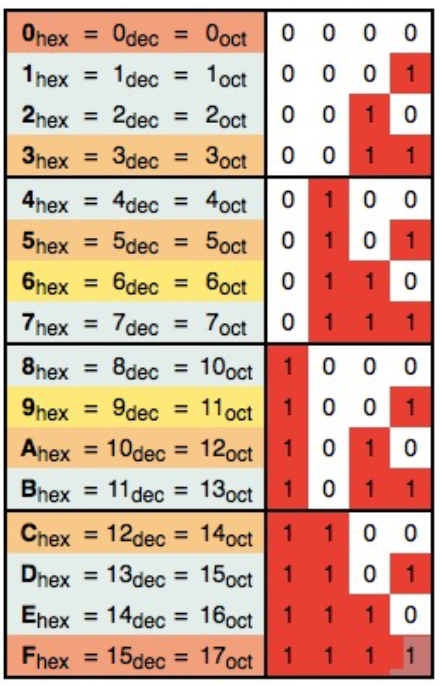
\includegraphics[width=60mm,scale=0.5]{confronto_tra_basi.png}    
\end{center}

\section{Conversione tra basi}
Svolti esercizi di conversione tra basi
\section{Operazioni aritmetiche e Overflow}
\begin{itemize}
    \item Addizzioni e sottrazioni
    \item Svolti esercizi con Overflow, bit di carry
\end{itemize}
 L'overflow di verifica quando il risultato non può essere rappresentato con il numero di bit,
 che ho a disposizione e quindi ottengo un risultato sbagliato.
\section{Operazioni con segno}
Ci sono diverse modalità per rappresentare il segno in base 2
\subsection{Modulo e segno}
La rappresentazione modulo e segno divide i bit di rappresentazione in 2, nel caso di 8 bit, 7 sono utilizzati per rappresentare il valore assoluto e il bit
più significativo (MSB - Most significant bit), quello a sinistra, rappresenta il segno, 0 positivo, 1 negativo
\begin{equation}
    1 | 0 0 0 0 1 0 0
\end{equation}
Questa rappresentazone è semplice e con n bit totali, si possono rappresentare i numeri interi nell'intervallo, ma ha alcuni problemi
\begin{itemize}
    \item Esistono 2 rappresentazioni diverse per lo 0
    \item Un bit tra tutti i bit disponibili viene speso per il segno e questo è uno spreco, riduce inoltre la capacità di rappresentazione
\end{itemize}

\subsection{Operazioni aritmetiche con MS}
Possiamo avere overflow solo quando:
\begin{itemize}
    \item si sommano due operandi con segno concorde
    \item si sottraggono due operandi con segno discorde
\end{itemize}
L'overflow si verifica quando c'è un riporto della cifra più significativa del modulo, cioè non si è nella
condizione di rappresentare il risultato ottenuto.
\subsection{Complemento a 1 (CA1)}
\'E un'altra modalità di rappresentazione dei numeri interi con segno. Come indica il nome stesso, questo metodo si basa sull'operazione di complemento

\paragraph{Complemento} è l'operazione che associa ad un bit (o ad ogni sequenza di bit) il suo opposto, cioè il valore ottento
sostituendo tutti gli 1 con 0 e uttti gli 0 con 1
\paragraph{Esecuzione} è semplice e diretta
\begin{enumerate}
    \item Se il numero da condificare è positivo lo si converte in binaro con il metodo tradizionale
    \item Sei il numero è negatio basta convertire in binario il suo modulo e quindi eseguire l'operazione di complemento sul numero appena convertito
\end{enumerate} 
\paragraph{Problema} ancora doppia rappresentazione dello 0

\subsection{Complemento a 2 (CA2)}
Anche qui il MSB è 0 se x è positivo e MSB = 1 se x è negativo
\paragraph{Esecuzione}
\begin{enumerate}
    \item Se il numero X è positivo esso rimane invariato
    \item Se il numero X è negativo
    \begin{enumerate}
        \item Si effettua il complemento a 1 (CA1) sul valore da codificare
        \item Si somma +1 al risultato ottenuto con CA1
    \end{enumerate}
\end{enumerate}
Così elimino la doppia rappresentazione dello zero. I valori negativi hanno MSB = 1.

\subsubsection{3 Metodi per il calcolo di CA2}
\begin{enumerate}
    \item Definizione di complemento alla base
    \item Per calcolare CA2 si calcola CA1 e si somma 1
    \item Regola Pratica
    \begin{enumerate}
        \item Si parte da destra, si trascrivono tutti gli 0 fino ad incontrare il primo 
        1 e si trascrive anch'esso
        \item Si complementano a 1 (0 $\to$ 1 e 1 $\to$ 0) tutti i bit restanti
    \end{enumerate}
\end{enumerate}

\title{Distinzione tra Operazione CA2 e Rappresentazone CA2}
\begin{itemize}
    \item La rappresentazione - come sono organizzati i bit
    \item Il calcolo - procedura di trasformazione
\end{itemize}

\subsection{Operazioni aritmetiche con CA2}
\subsubsection{Somma}
\begin{enumerate}
    \item Si esegue la somma su tutti i bit degli addendi, segno compreso
    \item Un eventuale riporto (carry) oltre il bit di segno (MSB) viene scartato
    \item Nel caso gli operandi siano di segno concorde occorre verificare la presenza o meno
    di overflow (il segno del risultato non  è concorde con quello dei due addendi)
\end{enumerate}
L'overflow non si presenta mai quando si sommano operandi di segno opposto.
L'overflow si presenta se:
\begin{equation}
    (+A)+(+B)=-C
\end{equation}
oppure
\begin{equation}
    (-A)+(-B) = +C    
\end{equation}
Un altro modo per vedere se c'è overflow è guardare i riporti nelle ultime 
due posizioni più significative, se sono diversi c'è overflow.
\subsubsection{Sottrazione}
La sottrazione tra 2 numeri in \textbf{CA2} viene trasformata in somma applicando la seguente Regola
\begin{equation}
    A-B=A+(-B)
\end{equation}
Tradotto in termini di CA2
\begin{equation}
    A-B=A+CA2(B)
\end{equation}
Si effettua il complemento del sottraendo
\paragraph{Overflow} Per assicurarsi della correttezza del risultato bisogna verificare l'assenza di 
Overflow:
\begin{enumerate}
    \item Non si ha overflow se gli operandi hanno segno discorde
    \item Si ha overflow se gli operandi hanno segno concorde e il segno del risultato è discorde con essi
\end{enumerate}
Gli operandi devono essere rappresentati sempre con lo stesso numero di bit, per questo motivo
in caso ci fossero meno bit si replica n volte il bit di segno (questo non altera il risultato)

\section{Operazione di Shift}
Consiste nello spostare (shit) verso destra (right) o verso sinistra (left) la posizione delle cifre di un numero, epsresso in una base qualsiasi, inserendo uno zero
nelle posizioni lasciate libere.
\begin{itemize}
    \item Left equivale a moltiplicare il numero per la base
    \item Right equivale a dividere il numero per la base
\end{itemize}
\section{Rappresentazione Eccesso $2^n$}
Un numero X è rappresentato come segue:
\begin{equation}
    X+2^{n-1}
\end{equation}
Con n bit si rappresenta l'eccesso
\paragraph{Regola pratica} I numeri in eccesso $2^{n-1}$ si ottengono da quelli in CA2
complementando il bit più significativo
\section{Rappresentazione Eccesso 128}
Il numero è rappresentato come segue
\begin{center}
    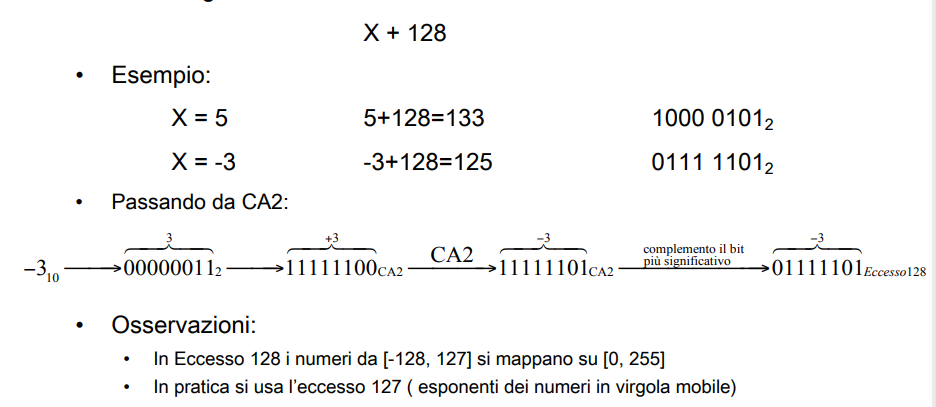
\includegraphics[width=120mm, scale=0.6]{eccesso128.png}
\end{center}

\section{Rappresentazione con la virgola}
\subsection{Virgola fissa}
\'E il metodo più semplice, scegliamo dove mettere la virgola e la fissiamo
Il problema è che in base a dove posiziono la virgola ho diverse capacità di rappresentazione della parte intera o frazionaria
\begin{itemize}
    \item Più a destra, scarsa rappresentazione intera, alta rappresentazione frazionaria
    \item Più a sinitra, scarsa rappresentazione frazionaria, alta rappresentazione intera
\end{itemize}
Questo porta rigidità

\subsection{Virgola mobile}
\begin{itemize}
    \item Usa 1 bit per rappresentare il segno s
    \item Usa altri bit per rappresentare la mantissa m
    \item Usa altri bit per codificare l'esponente e
\end{itemize}

Seguendo lo standard IEEE 754 la suddivisione è effettuata nella seguente modalità
\subsubsection{32 bit}
\begin{itemize}
    \item Segno - 1
    \item Esponente - 8
    \item Mantissa - 23
\end{itemize}
\subsubsection{64 bit}
\begin{itemize}
    \item Segno - 1
    \item Esponente - 11
    \item Mantissa - 52
\end{itemize}

\subsection{Errore assoluto ed errore relativo}
Rappresentando un numero reale n in virgola mobile si commette un errore di approssimazione,
dato che viene rappresentato un numero razionale n con un numero limitato di cifre significative
\begin{itemize}
    \item Errore assoluto
    \item Errore relativo
\end{itemize}
%Errore assoluto e relativo è Poco chiaro
\subsection{Codifiche}
Spiegazione ASCII, Unicode
%Aggiungere info

\chapter{Circuiti logici}

Nell'elettronica digitale sia ingressi che le uscite possono assumere solo i valori di sengale alto (1 per convenzione) o basso (0)

Un circuito o rete combinatoria è quel circuito

Un circuito o rete sequenziale

\section{Porte Logiche}
Le porte logiche sono i componenti elettronici che permettono di svolgere le operazioni logiche
primitive oltre che a quelle direttamente derivate.
Esse realizzano le operazioni principali dell'algebra booleana. Sono circuiti elettronici che dati dei segnali 0 e 1 in input
producono un segnale in output ottenuto effettuando una operazione booleana sugli ingressi.
Le porte logiche hanno n input e generalmente 1 output

\subsection{AND}
Questa porta logica svolge l'operazione logica di AND tra due bit, detta anche \textbf{prodotto logico}.
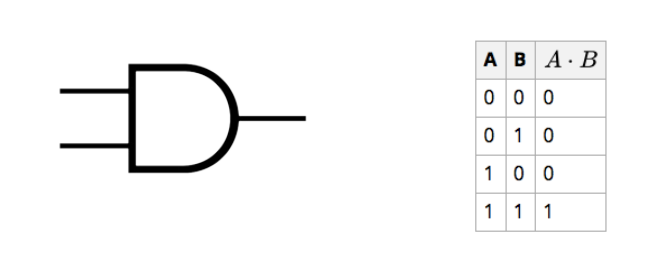
\includegraphics[width=100mm, scale=0.6]{tabella_and.png}

\subsection{OR}
Svolge l'operazione logica di OR tra due bit, detta anche somma logica.
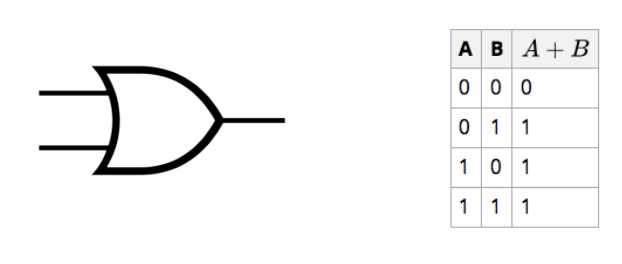
\includegraphics[width=100mm, scale=0.6]{tabella_or.png}

\subsection{NOT}
Svolge l'operazione logica di NOT su un bit, detta anche \textbf{negazione logica}.
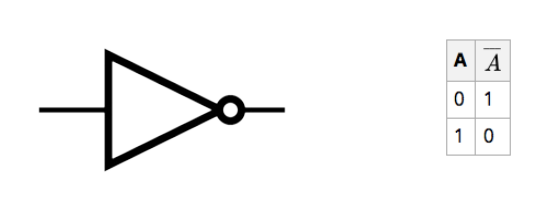
\includegraphics[width=100mm, scale=0.6]{tabella not.png}

\subsection{Port con più di due ingressi}
Ad eccezione della porta NOT, le altre porte logiche possono esistere anche ad N ingressi, queste porte
svolgono l'operazione logica associata su N bit invece che su 2.
\\ Nei circuiti si possono realizzare porte a N ingressi collegando a cascata tra loro porte a 2 ingressi.

\section{Porte logiche derivate}
Porta NAND $\to$ svolge l'operazione di NOT sul bit risultante dell'operazione di AND. 
(nega il risultato dell'and).
\\ Porta NOR $ \to $ svolge l'operazione di NOT sul bit risultante dall'operazione di OR.
(nega il risultato dell'or).
\\ Porta XOR Opera come disgiunzione esclusiva tra due input, quando i 2 bit sono uguali produce in output un 1. 
Viceversa restituisce 0.
Le porte NOR e NAND svolgono la funzione di inverter, sono definite universali

\section{Decoder}
Componente elettronico caratterizzato dall'avere n ingressi e $2^n$ uscite
Solo 1 valore è attivo per ogni combinazione di input, quindi l'ingresso seleziona 
una delle uscite, l'uscita selezionata ha valore 1 tutte le altre 0.
\\ Nella foto il pallino vuoto corrisponde a 0, mentre senza pallino corrisponde a 1.

\section{Multiplexor}
Un multiplexor, detto anche selettore, è un componente elettronico caratterizzato da
\begin{itemize}
    \item $2^n$ entrate principali
    \item n entrate di controllo (selettore)
    \item 1 uscite
\end{itemize}
Riceve n segnali in input e un solo segnale di output


\section{Logiche a due livelli e PLA}
Possiamo creare logiche a due livelli:
\begin{itemize}
    \item Somma di prodotti: somma logica (OR) di prodotti (AND)
    \item Prodotto di somme: prodotto (AND) di somme (OR)
\end{itemize}
Esercizio tabella di verità

\textbf{Programmable Logic Array}
La somma di prodotti corrisponde ad una implementazione comunemente nota come \textbf{Programmable Logic Array}
\begin{itemize}
    \item Insieme di input
    \item I corrispondenti input complementati (mediante inverter)
    \item Una logica a due stage:
    \begin{itemize}
        \item Primo stage: un array di porte logiche AND (prodotto)
        \item Secondo stage: un array di porte logiche OR (somma)
    \end{itemize}
\end{itemize}
\begin{center}
    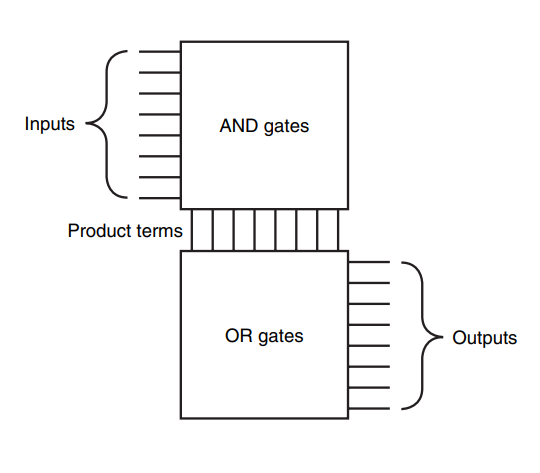
\includegraphics[width=70mm, scale=0.6]{ex_pla.png}    
\end{center}

\section{ROM (Read Only Memory)}
Circuito combinatorio in cui ad ogni ingresso (indirizzo)
corrisponde una uscita (contenuto della cella di memoria con quell'indirizzo).
\begin{itemize}
    \item Input: n bit
    \item Output: una tra le $2^n$ celle/locazioni di memoria
\end{itemize}

\paragraph{ROM vs PLA}
\begin{itemize}
    \item ROM - fully decoded VS PLA - partially decoded
    \item ROM dimensione più grande rispetto a PLA
    \item PLA più efficienti
    \item ROM possono implementare qualsiasi funzone logica
\end{itemize}

\begin{itemize}
    \item PROM (Programmable ROM) $\to$ possono essere programmate
    \item EPROM (Erasable Programmable ROM)
\end{itemize}

Normalmente il bus è di 32 bit

\section{ALU}
%Inserire descrizione ALU
Blocchi per la costruzione di una ALU
\begin{itemize}
    \item AND
    \item OR
\end{itemize}
Una Alu a 32 è semplicemente l'interconnessione di 32 ALU ad 1 bit in cascata
\section{BEQ: branch-on-equal}
\end{document}